\documentclass[conference]{IEEEtran}
\IEEEoverridecommandlockouts

\usepackage{cite}
\usepackage{amsmath,amssymb,amsfonts}
\usepackage{algorithmic}
\usepackage{graphicx}
\usepackage{textcomp}
\usepackage{xcolor}
\usepackage{booktabs}
\usepackage{hyperref}
\usepackage{multirow}
\usepackage{array}
\usepackage{CJKutf8}  % v1.2: Korean author support
% --- v1.1: TikZ figure support ---
\usepackage{tikz}
\usepackage{pgfplots}
\pgfplotsset{compat=1.18}
\usetikzlibrary{arrows.meta, shapes.geometric, positioning,
                fit, backgrounds, calc, decorations.pathreplacing}

\def\BibTeX{{\rm B\kern-.05em{\sc i\kern-.025em b}\kern-.08em
    T\kern-.1667em\lower.7ex\hbox{E}\kern-.125emX}}

\begin{document}

\title{Smartphone Camera-Based Multimodal Biomarker Framework for AI-Driven Prediction of PCOS and Endometriosis}

\author{\IEEEauthorblockN{\begin{CJK}{UTF8}{mj}신홍철\end{CJK} (Hongchul Shin)}
\IEEEauthorblockA{\begin{CJK}{UTF8}{mj}과학기술연합대학원대학교(U.S.T)\end{CJK}\\
University of Science and Technology (UST)\\
neohc@ust.ac.kr}}

\maketitle

\begin{abstract}
Polycystic ovary syndrome (PCOS) and endometriosis collectively affect over 300 million women worldwide, yet both conditions suffer from diagnostic delays averaging 7--10 years due to reliance on invasive procedures, hormonal assays, and specialist imaging. We propose the first smartphone camera-based multimodal biomarker framework specifically designed for non-invasive, AI-driven prediction of PCOS and endometriosis. Our framework integrates three complementary modalities: (1) remote photoplethysmography (rPPG)-derived heart rate variability (HRV), exploiting established autonomic nervous system dysregulation in both conditions (PCOS: LF/HF standardized mean difference $+0.670$, 17-study meta-analysis; endometriosis: significant RMSSD reduction); (2) facial and skin phenotype analysis using convolutional neural networks for acne grading (accuracy 0.85), hirsutism scoring (concordance 0.89), and acanthosis nigricans detection (AUC 0.854); and (3) longitudinal menstrual cycle tracking via app-reported data fused with HRV temporal patterns. We design a Cross-Attention Fusion architecture combining 1D-CNN/Transformer-extracted HRV features, EfficientNet-derived dermatological scores, and LSTM-encoded cycle features for three-class classification (PCOS/endometriosis/healthy), with an estimated macro-AUC of 0.80--0.90. A three-phase prospective cohort protocol (Phase~I: 150, Phase~II: 600, Phase~III: 300 participants) with Privacy-by-Design principles is proposed. We present a tiered biomarker evaluation across five dimensions, identifying four Tier~1 and six Tier~2 biomarkers. This work addresses a critical research gap at the intersection of smartphone sensing and women's reproductive health, offering a scalable pathway toward equitable early diagnosis.
\end{abstract}

\begin{IEEEkeywords}
PCOS, endometriosis, digital biomarker, smartphone camera, remote photoplethysmography, heart rate variability, multimodal AI, women's health
\end{IEEEkeywords}

%==============================================================================
\section{Introduction}
%==============================================================================

Polycystic ovary syndrome (PCOS) and endometriosis are the two most prevalent gynecological conditions affecting women of reproductive age, with estimated prevalences of 8--13\% and 6--10\%, respectively~\cite{Wang_2025, Pavic_2025}. Despite their high burden, both conditions are characterized by prolonged diagnostic delays. Endometriosis requires an average of 7--10 years from symptom onset to definitive diagnosis, typically via laparoscopy or advanced imaging~\cite{Zhang_2026}. PCOS diagnosis under the Rotterdam criteria demands ultrasound and hormonal assays, leaving a substantial proportion of affected women undiagnosed, particularly in resource-limited settings~\cite{Arabkermani_2025}.

The consequences of delayed diagnosis are severe. Untreated endometriosis leads to chronic pelvic pain, infertility, and reduced quality of life, while unmanaged PCOS increases risks of type~2 diabetes, cardiovascular disease, and endometrial cancer~\cite{Wang_2025}. The economic burden is substantial: endometriosis-related healthcare costs exceed \$12,000 per patient annually in the United States, and PCOS is associated with a 2.3-fold increase in healthcare utilization~\cite{Moghimikandelousi_2025}.

The global proliferation of smartphones---exceeding 6.9 billion users---presents an unprecedented opportunity for non-invasive, decentralized health screening. Modern smartphone cameras enable remote photoplethysmography (rPPG) for contactless extraction of heart rate variability (HRV) with correlations of $r=0.85$--$0.95$ against electrocardiogram (ECG) reference~\cite{rppgreview2024frontiers}. Simultaneously, deep learning advances have enabled automated analysis of skin conditions from smartphone images, including acne grading~\cite{Huynh_2022}, facial body mass index (BMI) estimation~\cite{Yousaf_2021}, and acanthosis nigricans detection~\cite{Dhanoo_2024}.

A critical research gap exists at the intersection of these technologies and women's reproductive health. While rPPG-based HRV has been extensively validated for cardiovascular monitoring~\cite{debnath2025comprehensive, luo2019smartphone}, and substantial evidence links autonomic dysregulation to both PCOS~\cite{Mirzohreh_2024} and endometriosis~\cite{Hao_2021, Moreira_2021}, no study has applied smartphone camera-based biomarkers to predict either condition. A recent comprehensive review of digital biomonitoring technologies for women's health~\cite{Moghimikandelousi_2025} confirms this void, identifying it as a priority area for future research.

This paper makes four contributions:
\begin{enumerate}
\item We present the first systematic evaluation of smartphone camera-based digital biomarkers specifically for PCOS and endometriosis prediction, identifying four Tier~1 and six Tier~2 candidate biomarkers through a five-dimensional assessment matrix.
\item We propose a novel multimodal AI framework integrating rPPG-HRV, facial skin phenotype analysis, and menstrual cycle data through Cross-Attention Fusion for three-class classification (PCOS/endometriosis/healthy).
\item We design a three-phase prospective cohort validation protocol (150$\rightarrow$600$\rightarrow$300 participants) with concrete sample size justifications grounded in meta-analytic effect sizes.
\item We address diagnostic equity by incorporating skin tone bias mitigation, Privacy-by-Design on-device processing, and accessibility considerations for underserved populations.
\end{enumerate}

%==============================================================================
\section{Related Work}
%==============================================================================

\subsection{rPPG-Based HRV Estimation}

Remote photoplethysmography extracts cardiovascular signals from facial video by detecting micro-variations in skin color caused by blood volume pulse. Debnath and Kim~\cite{debnath2025comprehensive} provide a comprehensive review documenting the evolution from signal processing methods (ICA, POS, CHROM) to deep learning architectures, with heart rate estimation achieving mean absolute error (MAE) of 0.5--3~bpm. Luo et al.~\cite{luo2019smartphone} demonstrated Transdermal Optical Imaging with 1,328 participants, achieving blood pressure estimation accuracy of 95.3\%/96.4\% for SBP/DBP within $\pm$5~mmHg. Cheng et al.~\cite{Cheng_2024} extended rPPG to contactless SpO$_2$ estimation using Spatial-Temporal Maps with CNN, achieving MAE of 1.274\% and RMSE of 1.710\%.

For HRV extraction specifically, a review of deep learning methods for rPPG~\cite{rppgreview2024frontiers} reported correlations of $r=0.85$--$0.95$ for time-domain (SDNN, RMSSD) and frequency-domain (LF, HF, LF/HF) metrics against ECG reference. The FibriCheck application~\cite{Sollee_2025} achieved FDA clearance for atrial fibrillation detection with 98.5\% accuracy, demonstrating clinical-grade performance from smartphone-based photoplethysmography. However, Acharya et al.~\cite{acharya2025reliability} identified that rPPG reliability degrades under low illumination and elevated heart rate, a critical consideration for real-world deployment in reproductive health monitoring.

\subsection{Facial and Skin Analysis for Disease Detection}

Deep learning applied to smartphone-captured skin images has achieved clinically relevant accuracy across multiple conditions. Huynh et al.~\cite{Huynh_2022} developed AcneDet, an automatic acne detection and severity grading system using smartphone images, achieving Investigator's Global Assessment (IGA) accuracy of 0.85. Gazeau et al.~\cite{Gazeau_2024} presented AcneAI at MICCAI 2024, reporting intraclass correlation coefficient (ICC) of 0.8 for automated acne severity assessment. Gao et al.~\cite{Gao_2025} further demonstrated large-scale acne evaluation with consistent performance across diverse skin types.

For BMI estimation, Yousaf et al.~\cite{Yousaf_2021} proposed semantic segmentation-based region-aware pooling from facial images, achieving MAE of 1.04, with particularly strong performance for women aged 21--40 (AUC 0.861 for overweight classification). Aarotale et al.~\cite{Aarotale_2023} introduced PatchBMI-Net for patch-based facial BMI estimation. Yolcu Oztel and Sahin~\cite{Oztel_2023} demonstrated skin lesion classification using DenseNet (92.25\%) and MobileNetV2 (98.4\%), establishing the feasibility of on-device dermatological analysis.

Dhanoo et al.~\cite{Dhanoo_2024} developed ANcam, a smartphone-based system for grading acanthosis nigricans using CMYK color channel analysis, achieving sensitivity of 81.1\%, specificity of 70.3\%, and AUC of 0.854 for detecting impaired glucose tolerance---directly relevant to PCOS-associated insulin resistance. Oliveira et al.~\cite{Oliveira_2022} validated image-based modified Ferriman-Gallwey (mFG) hirsutism scoring against in-person evaluation, demonstrating concordance of 0.89 and Cohen's $\kappa = 0.75$ in 70 participants, supporting remote PCOS phenotype assessment.

\subsection{PCOS and Endometriosis Digital Biomarkers}

The relationship between autonomic nervous system (ANS) dysfunction and PCOS is now established at meta-analytic strength. Mirzohreh et al.~\cite{Mirzohreh_2024} synthesized 17 studies demonstrating significantly altered HRV in PCOS: SDNN (SMD $-0.763$, 95\% CI: $-1.318$ to $-0.208$), LF/HF ratio (SMD $+0.670$, 95\% CI: $0.207$ to $1.133$), HFnu (SMD $-0.873$, 95\% CI: $-1.472$ to $-0.274$), and total HRV power (SMD $-1.997$, 95\% CI: $-3.437$ to $-0.557$). Yu et al.~\cite{Yu_2024} reviewed the role of ANS in PCOS pathophysiology, identifying sympathetic overactivation as both a consequence and contributor to hyperandrogenism. Individual studies further confirm these patterns: Sarathivarman et al.~\cite{Sarathivarman_2025} demonstrated significant HRV differences in PCOS women, de Fatima Azevedo et al.~\cite{de_Fatima_Azevedo_2026} linked PCOS to 24-hour blood pressure alterations, and Bernal et al.~\cite{Bernal_2024} showed that aerobic training partially reversed sympathetic autonomic modulation abnormalities in PCOS with excess body fat.

For endometriosis, multiple studies have identified vagal tone reduction. Hao et al.~\cite{Hao_2021} reported significantly reduced vagal tone in endometriosis patients and proposed auricular vagus nerve stimulation as therapeutic. Moreira et al.~\cite{Moreira_2021} demonstrated significant associations between pain severity, perceived stress, and vagally-mediated HRV (vmHRV) in endometriosis. Zeng et al.~\cite{Zeng_2025} confirmed reduced vagal tone in adenomyosis, a closely related condition. Moreira et al.~\cite{Moreira_2024} further showed that mindfulness-based intervention improved HRV and reduced pain in endometriosis, suggesting HRV as both a biomarker and therapeutic target.

The menstrual cycle modulates HRV in predictable patterns that are disrupted in PCOS. De Jager et al.~\cite{de_Jager_2026} conducted a living systematic review of wearable-derived HRV across the menstrual cycle, establishing phase-dependent variation in healthy women. Heydari et al.~\cite{Heydari_2025} proposed a new metric linking HRV to menstrual regularity using large-scale digital data from \textit{npj Digital Medicine}. Rajesh~\cite{Rajesh_2025} demonstrated a contactless menstrual health prediction framework using PPG achieving 91.7\% accuracy for cycle phase classification and 87.6\% for irregular cycles.

Wang et al.~\cite{Wang_2025} comprehensively reviewed AI applications in PCOS management, reporting 80--90\% diagnostic accuracy across various modalities, while Zhang et al.~\cite{Zhang_2026} conducted a meta-analysis of machine learning for endometriosis diagnosis. Liu et al.~\cite{Liu_2025} demonstrated that integrating inflammatory biomarkers with machine learning improves endometriosis risk prediction. However, none of these studies employed smartphone camera-based biomarkers, confirming the research gap our framework addresses.

%==============================================================================
\section{Proposed Multimodal Framework}
%==============================================================================

\subsection{System Architecture Overview}

The proposed framework consists of four interconnected modules operating in a pipeline architecture (Fig.~\ref{fig:arch}). The smartphone serves as the sole data collection device, with three input streams: (1) a 60-second frontal facial video captured by the front-facing camera for rPPG-HRV extraction; (2) three standardized selfie photographs (frontal, left 45\textdegree, right 45\textdegree) for facial and skin phenotype analysis; and (3) daily menstrual cycle tracking data entered via a companion mobile application. Each module extracts a fixed-dimensional feature vector, which the Cross-Attention Fusion layer integrates for final three-class prediction. On-device processing ensures that raw images and video are never transmitted to external servers, adhering to Privacy-by-Design principles.

% ── Fig. 1: System Architecture (two-column wide) ──────────────────────────
\begin{figure*}[t]
\centering
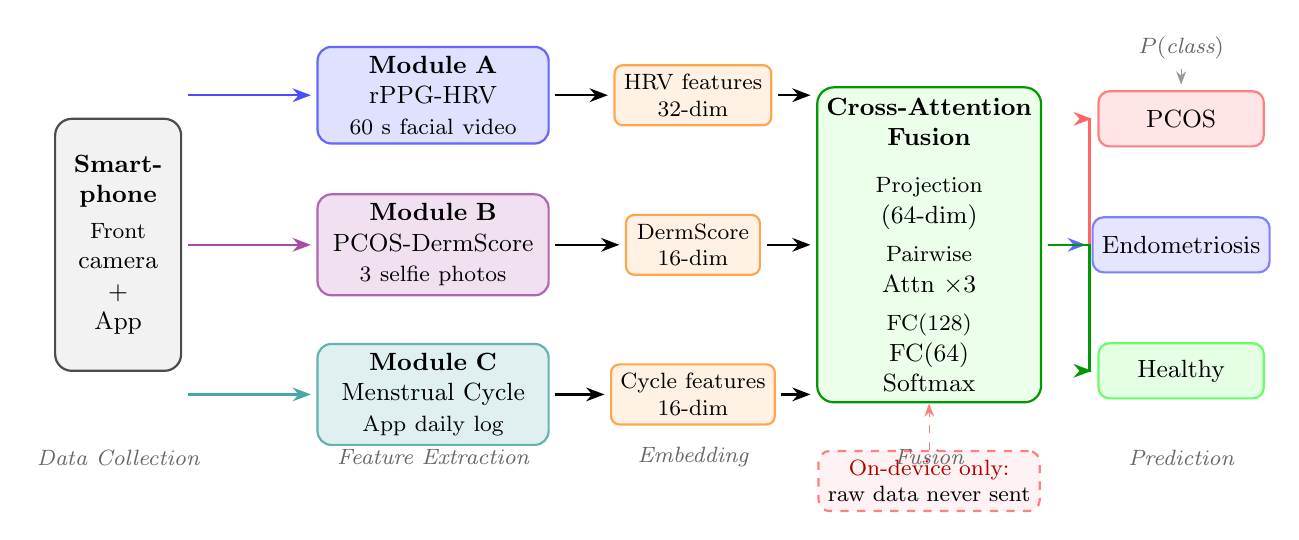
\begin{tikzpicture}[
  >=Stealth,
  thick,
  font=\small,
  phonebox/.style={
    draw=black!70, fill=gray!10, rounded corners=6pt,
    minimum width=1.6cm, minimum height=3.2cm, align=center
  },
  modbox/.style={
    draw, rounded corners=5pt,
    minimum width=2.9cm, minimum height=1.1cm,
    align=center, text width=2.7cm
  },
  modA/.style={modbox, fill=blue!12, draw=blue!60},
  modB/.style={modbox, fill=violet!12, draw=violet!60},
  modC/.style={modbox, fill=teal!12, draw=teal!60},
  featbox/.style={
    draw=orange!70, fill=orange!10, rounded corners=3pt,
    minimum width=1.7cm, minimum height=0.75cm,
    align=center, font=\footnotesize
  },
  fusbox/.style={
    draw=green!60!black, fill=green!8, rounded corners=6pt,
    minimum width=2.5cm, minimum height=4.0cm,
    align=center
  },
  outbox/.style={
    draw, rounded corners=4pt,
    minimum width=2.1cm, minimum height=0.7cm,
    align=center, font=\small
  },
  privbox/.style={
    draw=red!50, fill=red!5, rounded corners=4pt,
    minimum width=2.1cm, minimum height=0.6cm,
    align=center, font=\footnotesize, dashed
  },
  arr/.style={->, thick, shorten >=2pt, shorten <=2pt},
  labl/.style={font=\footnotesize\itshape, text=black!60}
]

\node[phonebox] (phone) at (0, 0) {
  \textbf{Smart-}\\
  \textbf{phone}\\[2pt]
  \footnotesize Front\\camera\\+\\App
};

\node[modA] (modA) at (4.0, 1.9) {
  \textbf{Module A}\\rPPG-HRV\\{\footnotesize 60 s facial video}
};
\node[modB] (modB) at (4.0, 0.0) {
  \textbf{Module B}\\PCOS-DermScore\\{\footnotesize 3 selfie photos}
};
\node[modC] (modC) at (4.0, -1.9) {
  \textbf{Module C}\\Menstrual Cycle\\{\footnotesize App daily log}
};

\node[featbox] (fA) at (7.3, 1.9) {HRV features\\32-dim};
\node[featbox] (fB) at (7.3, 0.0) {DermScore\\16-dim};
\node[featbox] (fC) at (7.3,-1.9) {Cycle features\\16-dim};

\node[fusbox] (fusion) at (10.3, 0.0) {
  \textbf{Cross-Attention}\\
  \textbf{Fusion}\\[6pt]
  \footnotesize Projection\\(64-dim)\\[3pt]
  \footnotesize Pairwise\\Attn $\times 3$\\[3pt]
  \footnotesize FC(128)\\FC(64)\\Softmax
};

\node[outbox, fill=red!10,   draw=red!50]   (o1) at (13.5, 1.6) {PCOS};
\node[outbox, fill=blue!10,  draw=blue!50]  (o2) at (13.5, 0.0) {Endometriosis};
\node[outbox, fill=green!10, draw=green!60] (o3) at (13.5,-1.6) {Healthy};

\node[privbox] (priv) at (10.3, -3.0) {%
  \textcolor{red!70!black}{On-device only:}\\raw data never sent
};

\draw[arr, blue!70]   (phone.east |- modA.west) -- (modA.west);
\draw[arr, violet!70] (phone.east |- modB.west) -- (modB.west);
\draw[arr, teal!70]   (phone.east |- modC.west) -- (modC.west);

\draw[arr] (modA.east) -- (fA.west);
\draw[arr] (modB.east) -- (fB.west);
\draw[arr] (modC.east) -- (fC.west);

\draw[arr] (fA.east) -- (fusion.west |- fA.east);
\draw[arr] (fB.east) -- (fusion.west);
\draw[arr] (fC.east) -- (fusion.west |- fC.east);

\draw[arr, red!60]   (fusion.east) -- ++(0.6,0) |- (o1.west);
\draw[arr, blue!60]  (fusion.east) -- ++(0.6,0) |- (o2.west);
\draw[arr, green!60!black] (fusion.east) -- ++(0.6,0) |- (o3.west);

\draw[->, dashed, red!50, thin] (priv.north) -- (fusion.south);

\node[labl] at (13.5, 2.5) {$P(\text{class})$};
\draw[arr, black!40, thin] (13.5, 2.3) -- (o1.north);

\node[labl] at (0,   -2.7) {Data Collection};
\node[labl] at (4.0, -2.7) {Feature Extraction};
\node[labl] at (7.3, -2.7) {Embedding};
\node[labl] at (10.3,-2.7) {Fusion};
\node[labl] at (13.5,-2.7) {Prediction};

\end{tikzpicture}
\caption{System architecture of the proposed multimodal smartphone camera-based framework.
Three independent modules extract complementary feature vectors from a single smartphone.
The Cross-Attention Fusion layer learns pairwise inter-modal interactions before
three-class softmax classification. On-device processing ensures that raw biometric
data are never transmitted to external servers.}
\label{fig:arch}
\end{figure*}
% ────────────────────────────────────────────────────────────────────────────

\subsection{Biomarker Collection Protocol}

\subsubsection{Module A: rPPG-HRV Extraction}
The user records a 60-second facial video using the smartphone front camera (minimum 8~MP, iOS~15+ or Android~11+) under indoor lighting conditions (50--500 lux). Face detection employs MediaPipe Face Mesh (468 landmarks) optimized for mobile deployment. Regions of interest (ROIs) are selected from the forehead and bilateral cheeks across RGB channels. The rPPG signal is extracted using a hybrid approach: CHROM (Chrominance-based method) for robustness under varying illumination, supplemented by DeepPhys for improved performance in low-light conditions. Inter-beat intervals (IBIs) are detected from the rPPG waveform, followed by standard HRV computation: time-domain metrics (SDNN, RMSSD, pNN50, meanRR) and frequency-domain metrics (LF power, HF power, LF/HF ratio, HFnu). A Signal Quality Index (SQI) is computed automatically; sessions with SQI~$<$~0.6 trigger a re-recording prompt. Measurements are performed once daily (morning, pre-caffeine) for longitudinal pattern capture.

\subsubsection{Module B: Facial Skin Phenotype Analysis (PCOS-DermScore)}
Three standardized photographs are captured weekly under consistent lighting. Four sub-modules operate in parallel: (1)~\textit{Acne Detection and Grading}: a Faster R-CNN detector localizes lesions, followed by classification into IGA grades 0--4 using a LightGBM ensemble, building on the AcneDet architecture~\cite{Huynh_2022}; (2)~\textit{Hirsutism Scoring}: a ResNet50 regression model estimates the modified Ferriman-Gallwey (mFG) score from upper lip, chin, and neck regions, validated against the image-based protocol of Oliveira et al.~\cite{Oliveira_2022}; (3)~\textit{Acanthosis Nigricans Detection}: CMYK color channel analysis of neck photographs following the ANcam methodology~\cite{Dhanoo_2024} classifies AN presence and severity; (4)~\textit{Facial BMI Estimation}: ResNet50 with semantic segmentation-based pooling~\cite{Yousaf_2021} provides continuous BMI estimation. The four outputs are concatenated into a 16-dimensional DermScore feature vector.

\subsubsection{Module C: Menstrual Cycle Pattern Analysis}
Participants record daily data via the companion application: cycle day, bleeding status and intensity, pain visual analog scale (VAS, 0--100~mm), mood, and energy level. Historical data spanning at least six cycles are processed through a two-layer LSTM network (hidden dimension 64) to extract cycle regularity features, while a Temporal Convolutional Network (TCN) encodes pain temporal patterns. A Transformer Encoder generates a symptom profile embedding from multivariate daily records. The combined output is a 16-dimensional cycle feature vector. Missing data are handled through learned masking, with a minimum recording threshold of 70\% of cycle days required for inclusion.

\subsection{AI Model Design: Cross-Attention Fusion}

The three feature vectors---HRV (32-dimensional), DermScore (16-dimensional), and Cycle (16-dimensional)---are projected into a shared 64-dimensional embedding space. The Cross-Attention Fusion mechanism computes pairwise attention between modalities:

\begin{equation}
\text{Attn}(Q_i, K_j, V_j) = \text{softmax}\left(\frac{Q_i K_j^T}{\sqrt{d_k}}\right) V_j
\end{equation}

\noindent where $Q_i$ is the query from modality $i$, and $K_j$, $V_j$ are the key and value from modality $j$. This enables the model to learn inter-modal interactions---for instance, how HRV patterns modulate the diagnostic significance of skin phenotype features. The fused representation passes through two fully connected layers (dimensions 128 and 64) with dropout ($p = 0.3$) before a softmax output layer producing three-class probabilities: PCOS, endometriosis, and healthy.

% ── Fig. 3: Cross-Attention Fusion detail (single column) ──────────────────
\begin{figure}[t]
\centering
\begin{tikzpicture}[
  >=Stealth, font=\footnotesize, thick,
  vec/.style={draw, rounded corners=3pt,
              minimum width=1.8cm, minimum height=0.55cm,
              align=center},
  proj/.style={draw, fill=gray!10, rounded corners=3pt,
               minimum width=1.8cm, minimum height=0.55cm,
               align=center},
  attn/.style={draw, fill=yellow!15, rounded corners=4pt,
               minimum width=1.8cm, minimum height=0.7cm,
               align=center},
  fc/.style={draw, fill=green!10, rounded corners=3pt,
             minimum width=3.8cm, minimum height=0.55cm,
             align=center},
  out/.style={draw, rounded corners=3pt,
              minimum width=1.1cm, minimum height=0.55cm,
              align=center},
  arr/.style={->, shorten >=1.5pt, shorten <=1.5pt}
]

\node[vec, fill=blue!12,   draw=blue!60]   (hA) at (0, 3.6) {HRV $\mathbf{h}_A$\\32-dim};
\node[vec, fill=violet!12, draw=violet!60] (hB) at (0, 2.2) {Derm $\mathbf{h}_B$\\16-dim};
\node[vec, fill=teal!12,   draw=teal!60]   (hC) at (0, 0.8) {Cycle $\mathbf{h}_C$\\16-dim};

\node[proj] (pA) at (2.4, 3.6) {Linear\\64-dim};
\node[proj] (pB) at (2.4, 2.2) {Linear\\64-dim};
\node[proj] (pC) at (2.4, 0.8) {Linear\\64-dim};

\node[attn] (atAB) at (4.6, 4.0) {Attn\\$A{\to}B$};
\node[attn] (atAC) at (4.6, 3.2) {Attn\\$A{\to}C$};
\node[attn] (atBA) at (4.6, 2.5) {Attn\\$B{\to}A$};
\node[attn] (atBC) at (4.6, 1.8) {Attn\\$B{\to}C$};
\node[attn] (atCA) at (4.6, 1.1) {Attn\\$C{\to}A$};
\node[attn] (atCB) at (4.6, 0.4) {Attn\\$C{\to}B$};

\node[fc, fill=green!12] (fc1) at (2.4,-0.6) {Concat + FC(128) + ReLU};
\node[fc, fill=green!18] (fc2) at (2.4,-1.4) {FC(64) + ReLU + Drop(0.3)};

\node[out, fill=red!10,   draw=red!50]   (o1) at (0.6, -2.4) {PCOS};
\node[out, fill=blue!10,  draw=blue!50]  (o2) at (2.4, -2.4) {Endo};
\node[out, fill=green!10, draw=green!60] (o3) at (4.2, -2.4) {Healthy};

\node[draw, dashed, rounded corners=3pt,
      minimum width=3.8cm, minimum height=0.55cm,
      align=center, font=\footnotesize] (sm)
  at (2.4,-1.95) {Softmax};

\draw[arr, blue!60]   (hA)--(pA);
\draw[arr, violet!60] (hB)--(pB);
\draw[arr, teal!60]   (hC)--(pC);

\draw[arr] (pA.east) -- ++(0.2,0) |- (atAB.west);
\draw[arr] (pA.east) -- ++(0.2,0) |- (atAC.west);
\draw[arr] (pB.east) -- ++(0.1,0) |- (atBA.west);
\draw[arr] (pB.east) -- ++(0.1,0) |- (atBC.west);
\draw[arr] (pC.east) -- ++(0.1,0) |- (atCA.west);
\draw[arr] (pC.east) -- ++(0.1,0) |- (atCB.west);

\foreach \n in {atAB,atAC,atBA,atBC,atCA,atCB}{
  \draw[arr, gray!60] (\n.south) |- (fc1.east);
}

\draw[arr] (fc1)--(fc2);
\draw[arr] (fc2)--(sm);
\draw[arr] (sm.south) -- ++(0,-0.15) -| (o1.north);
\draw[arr] (sm.south) -- ++(0,-0.15) -| (o2.north);
\draw[arr] (sm.south) -- ++(0,-0.15) -| (o3.north);

\node[draw=red!40, dashed, fill=red!4, rounded corners=3pt,
      align=center, font=\tiny, text width=3.5cm]
  (miss) at (2.4, -3.3)
  {Missing modality: attention weights\\redistribute to available modalities};
\draw[->, dashed, red!40, thin] (miss.north)--(sm.south);

\end{tikzpicture}
\caption{Cross-Attention Fusion architecture detail.
Each modality pair computes bidirectional attention ($A{\to}B$, $B{\to}A$, etc.),
yielding six attention outputs that are concatenated and passed through two
fully connected layers before softmax classification.
When a modality is unavailable, attention weights redistribute automatically,
enabling prediction from partial inputs.}
\label{fig:fusion}
\end{figure}
% ────────────────────────────────────────────────────────────────────────────

A key advantage of Cross-Attention Fusion over simple concatenation is its ability to handle missing modalities gracefully. When a modality is unavailable (e.g., insufficient menstrual data in early enrollment), attention weights redistribute to available modalities, enabling prediction from partial data.

Training employs a two-stage strategy: (1) each module is pre-trained independently on public datasets (UBFC-rPPG for Module~A, ACNE04 for acne detection, CelebA for BMI estimation); (2) the full model is fine-tuned end-to-end on the collected cohort data using 5-fold stratified cross-validation with a held-out 20\% test set. Model interpretability is ensured through SHAP values for feature importance and Grad-CAM for spatial attention visualization. On-device deployment uses TensorFlow Lite (Android) and Core ML (iOS), with inference time targeted at $<$5~seconds per session.

\subsection{Evaluation Design: Three-Phase Cohort Protocol}

\subsubsection{Study Population}
The target population comprises reproductive-age women (18--45 years) with smartphone ownership (front camera $\geq$8~MP). Three groups are enrolled: PCOS (Rotterdam criteria-confirmed via ultrasound and hormonal assays), endometriosis (laparoscopy/MRI/ultrasound-confirmed, rASRM stages I--IV), and healthy controls (regular menstruation, no gynecological history). Exclusion criteria include PCOS-endometriosis comorbidity, hormonal contraceptive use within 3 months, cardiovascular or autonomic disorders, and active dermatological treatment.

\subsubsection{Phase I: Feasibility Pilot (6 months, $n=150$)}
Fifty participants per group undergo the full biomarker collection protocol. Primary objectives are technical validation of rPPG-HRV against simultaneous ECG recording ($n=50$ subset) and preliminary effect size estimation for sample size refinement.

\subsubsection{Phase II: Validation Cohort (12--18 months, $n=600$)}
Two hundred participants per group, powered by the meta-analytic effect size of $d=0.57$ for PCOS-HRV differences~\cite{Mirzohreh_2024} with 15\% attenuation for rPPG conversion, $\alpha=0.05$, and power 0.80, plus 20\% dropout allowance. For the machine learning model (approximately 50 features), the empirical rule of $\geq$10 cases per feature yields a minimum of 500 total participants. This phase tests all five hypotheses and develops the multimodal classification model.

\subsubsection{Phase III: External Validation (6 months, $n=300$)}
One hundred participants per group at independent clinical sites provide external generalizability assessment, including cross-site, cross-device, and cross-ethnicity validation.

% ── Fig. 4: Three-Phase Cohort Timeline (two-column wide) ──────────────────
\begin{figure*}[t]
\centering
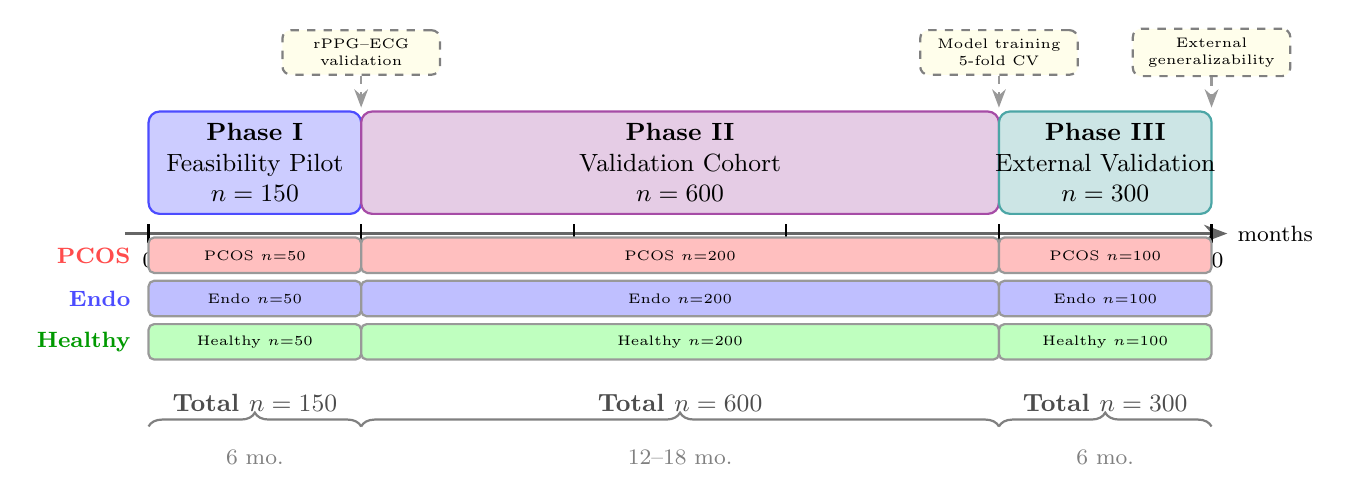
\begin{tikzpicture}[
  >=Stealth, font=\small, thick,
  phasebox/.style={draw, rounded corners=5pt,
                   minimum height=1.1cm, align=center},
  grpbox/.style={draw, rounded corners=3pt,
                 minimum width=1.4cm, minimum height=0.65cm,
                 align=center, font=\footnotesize},
  milestonebox/.style={draw=black!50, dashed, rounded corners=3pt,
                        minimum width=2.0cm, minimum height=0.5cm,
                        align=center, font=\tiny, fill=yellow!8}
]

\def\TW{13.5}
\def\TY{0}
\def\Tstart{0}
\def\Tend{30}

\draw[->, very thick, black!60] (-0.3, \TY) -- (\TW+0.2, \TY);
\node[right, font=\footnotesize] at (\TW+0.2, \TY) {months};

\foreach \m/\lab in {0/0, 6/6, 12/12, 18/18, 24/24, 30/30}{
  \pgfmathsetmacro\x{\m/\Tend*\TW}
  \draw (\x, 0.12)--(\x,-0.12);
  \node[below, font=\footnotesize] at (\x,-0.12) {\lab};
}

\pgfmathsetmacro\pIx{0}
\pgfmathsetmacro\pIw{6/\Tend*\TW}
\filldraw[fill=blue!20, draw=blue!70, rounded corners=4pt]
  (\pIx, 0.25) rectangle (\pIx+\pIw, 1.55);
\node[align=center, font=\small] at (\pIx+\pIw/2, 0.9) {
  \textbf{Phase~I}\\Feasibility Pilot\\$n=150$
};

\pgfmathsetmacro\pIIx{6/\Tend*\TW}
\pgfmathsetmacro\pIIw{18/\Tend*\TW}
\filldraw[fill=violet!20, draw=violet!70, rounded corners=4pt]
  (\pIIx, 0.25) rectangle (\pIIx+\pIIw, 1.55);
\node[align=center, font=\small] at (\pIIx+\pIIw/2, 0.9) {
  \textbf{Phase~II}\\Validation Cohort\\$n=600$
};

\pgfmathsetmacro\pIIIx{24/\Tend*\TW}
\pgfmathsetmacro\pIIIw{6/\Tend*\TW}
\filldraw[fill=teal!20, draw=teal!70, rounded corners=4pt]
  (\pIIIx, 0.25) rectangle (\pIIIx+\pIIIw, 1.55);
\node[align=center, font=\small] at (\pIIIx+\pIIIw/2, 0.9) {
  \textbf{Phase~III}\\External Validation\\$n=300$
};

\foreach \g/\col/\yy in {PCOS/red!25/-0.5, Endo/blue!25/-1.05, Healthy/green!25/-1.6}{
  \filldraw[fill=\col, draw=black!40, rounded corners=2pt]
    (0, \yy) rectangle (\pIw, \yy+0.45);
  \node[font=\tiny, align=center] at (\pIw/2, \yy+0.22) {\g\ $n{=}50$};
}

\foreach \g/\col/\yy in {PCOS/red!25/-0.5, Endo/blue!25/-1.05, Healthy/green!25/-1.6}{
  \filldraw[fill=\col, draw=black!40, rounded corners=2pt]
    (\pIIx, \yy) rectangle (\pIIx+\pIIw, \yy+0.45);
  \node[font=\tiny, align=center] at (\pIIx+\pIIw/2, \yy+0.22) {\g\ $n{=}200$};
}

\foreach \g/\col/\yy in {PCOS/red!25/-0.5, Endo/blue!25/-1.05, Healthy/green!25/-1.6}{
  \filldraw[fill=\col, draw=black!40, rounded corners=2pt]
    (\pIIIx, \yy) rectangle (\pIIIx+\pIIIw, \yy+0.45);
  \node[font=\tiny, align=center] at (\pIIIx+\pIIIw/2, \yy+0.22) {\g\ $n{=}100$};
}

\node[left, font=\footnotesize\bfseries, text=red!70]    at (-0.1,-0.28) {PCOS};
\node[left, font=\footnotesize\bfseries, text=blue!70]   at (-0.1,-0.83) {Endo};
\node[left, font=\footnotesize\bfseries, text=green!60!black] at (-0.1,-1.38) {Healthy};

\pgfmathsetmacro\mIend{6/\Tend*\TW}
\pgfmathsetmacro\mIIend{24/\Tend*\TW}
\pgfmathsetmacro\mIIIend{30/\Tend*\TW}

\node[milestonebox] (ms1) at (\mIend,   2.3) {rPPG--ECG\\validation};
\node[milestonebox] (ms2) at (\mIIend,  2.3) {Model training\\5-fold CV};
\node[milestonebox] (ms3) at (\mIIIend, 2.3) {External\\generalizability};

\draw[->, dashed, black!40] (ms1.south)--(\mIend, 1.6);
\draw[->, dashed, black!40] (ms2.south)--(\mIIend, 1.6);
\draw[->, dashed, black!40] (ms3.south)--(\mIIIend, 1.6);

\node[font=\small\bfseries, text=black!70] at (\pIw/2,    -2.15) {Total $n=150$};
\node[font=\small\bfseries, text=black!70] at (\pIIx+\pIIw/2, -2.15) {Total $n=600$};
\node[font=\small\bfseries, text=black!70] at (\pIIIx+\pIIIw/2,-2.15){Total $n=300$};

\draw[decorate, decoration={brace,amplitude=5pt}, black!50]
  (0, -2.45) -- (\pIw, -2.45)
  node[midway, below=5pt, font=\footnotesize] {6 mo.};
\draw[decorate, decoration={brace,amplitude=5pt}, black!50]
  (\pIIx, -2.45) -- (\pIIx+\pIIw, -2.45)
  node[midway, below=5pt, font=\footnotesize] {12--18 mo.};
\draw[decorate, decoration={brace,amplitude=5pt}, black!50]
  (\pIIIx, -2.45) -- (\pIIIx+\pIIIw, -2.45)
  node[midway, below=5pt, font=\footnotesize] {6 mo.};

\end{tikzpicture}
\caption{Three-phase prospective cohort protocol.
Phase~I ($n=150$, 6 months) validates rPPG-HRV against ECG reference and estimates
effect sizes. Phase~II ($n=600$, 12--18 months) is powered at $\alpha=0.05$,
$1-\beta=0.80$ for the meta-analytic HRV effect size ($d=0.57$) with 20\% dropout
allowance, and trains the multimodal classification model.
Phase~III ($n=300$, 6 months) provides external generalizability testing
across independent sites, devices, and ethnicities.}
\label{fig:cohort}
\end{figure*}
% ────────────────────────────────────────────────────────────────────────────

%==============================================================================
\section{Biomarker Evaluation Results}
%==============================================================================

\subsection{Tier Classification}

We evaluated candidate biomarkers using a five-dimensional scoring matrix: Technical Readiness Level (TRL), Clinical Validity (CV), Practicality (PR), Data Availability (DA), and Regulatory Friendliness (RF), each scored 1--5. Biomarkers scoring $\geq$18 were classified as Tier~1 (directly applicable), 13--17 as Tier~2 (promising with additional validation needed), and 7--12 as Tier~3 (exploratory). Table~\ref{tab:tier} presents the classification results.

\begin{table*}[t]
\centering
\caption{Tiered Classification of Smartphone Camera-Based Biomarkers for PCOS and Endometriosis}
\label{tab:tier}
\begin{tabular}{llllccccccc}
\toprule
\textbf{Tier} & \textbf{Biomarker} & \textbf{Disease} & \textbf{Best Performance} & \textbf{TRL} & \textbf{CV} & \textbf{PR} & \textbf{DA} & \textbf{RF} & \textbf{Total} \\
\midrule
\multirow{4}{*}{1} & rPPG-HRV (LF/HF, RMSSD, HFnu) & PCOS + Endo & ECG $r$=0.85--0.95; LF/HF SMD +0.670 & 4 & 5 & 5 & 4 & 3 & \textbf{21} \\
 & Menstrual Cycle HRV Pattern & PCOS & RF AUC 0.96 (wearable) & 3 & 4 & 5 & 4 & 3 & \textbf{19} \\
 & Acne Auto-grading (IGA) & PCOS & IGA accuracy 0.85, mAP 0.54 & 4 & 4 & 5 & 3 & 3 & \textbf{19} \\
 & Hirsutism Image mFG Score & PCOS & Concordance 0.89, $\kappa$=0.75 & 3 & 4 & 5 & 3 & 3 & \textbf{18} \\
\midrule
\multirow{6}{*}{2} & Acanthosis Nigricans (ANcam) & PCOS & Sens 81.1\%, Spec 70.3\%, AUC 0.854 & 3 & 3 & 4 & 3 & 4 & \textbf{17} \\
 & Facial BMI Estimation & PCOS & MAE 1.04, AUC 0.861 & 4 & 3 & 5 & 2 & 2 & \textbf{16} \\
 & rPPG Blood Pressure (SBP/DBP) & PCOS & 95.3\%/96.4\% ($\pm$5mmHg) & 3 & 3 & 5 & 3 & 2 & \textbf{16} \\
 & rPPG SpO$_2$ Estimation & Endo & MAE 1.274\%, RMSE 1.710\% & 3 & 3 & 5 & 2 & 2 & \textbf{15} \\
 & Contactless Menstrual 4-Phase & PCOS & PPG 91.7\%, irregular 87.6\% & 2 & 3 & 5 & 2 & 2 & \textbf{14} \\
 & Skin Lesion Classification & PCOS & DenseNet 92.25\%, MobileNet 98.4\% & 4 & 2 & 5 & 2 & 1 & \textbf{14} \\
\midrule
\multirow{4}{*}{3} & Skin Color Time-series (L*a*b*) & PCOS & Hypothesis-level & 2 & 2 & 4 & 2 & 1 & \textbf{11} \\
 & Micro-expression + rPPG Pain & Endo & Hypothesis-level & 2 & 2 & 3 & 2 & 1 & \textbf{10} \\
 & Nocturnal rPPG SpO$_2$ & PCOS-OSA & Hypothesis-level & 1 & 2 & 3 & 2 & 1 & \textbf{9} \\
 & Androgenetic Alopecia Pattern & PCOS & Hypothesis-level & 1 & 2 & 3 & 1 & 1 & \textbf{8} \\
\bottomrule
\end{tabular}
\end{table*}

Four Tier~1 biomarkers were identified, all scoring $\geq$18/25. The highest-ranked biomarker, rPPG-HRV (total score 21), benefits from both high clinical validity (meta-analytic evidence for both PCOS and endometriosis) and high technical maturity (rPPG-ECG correlation $r=0.85$--$0.95$). Notably, all Tier~1 biomarkers are collectible using a standard smartphone camera without additional hardware.

% ── Fig. 2: Tier 1 Radar Chart (two-column wide) ───────────────────────────
\begin{figure*}[t]
\centering
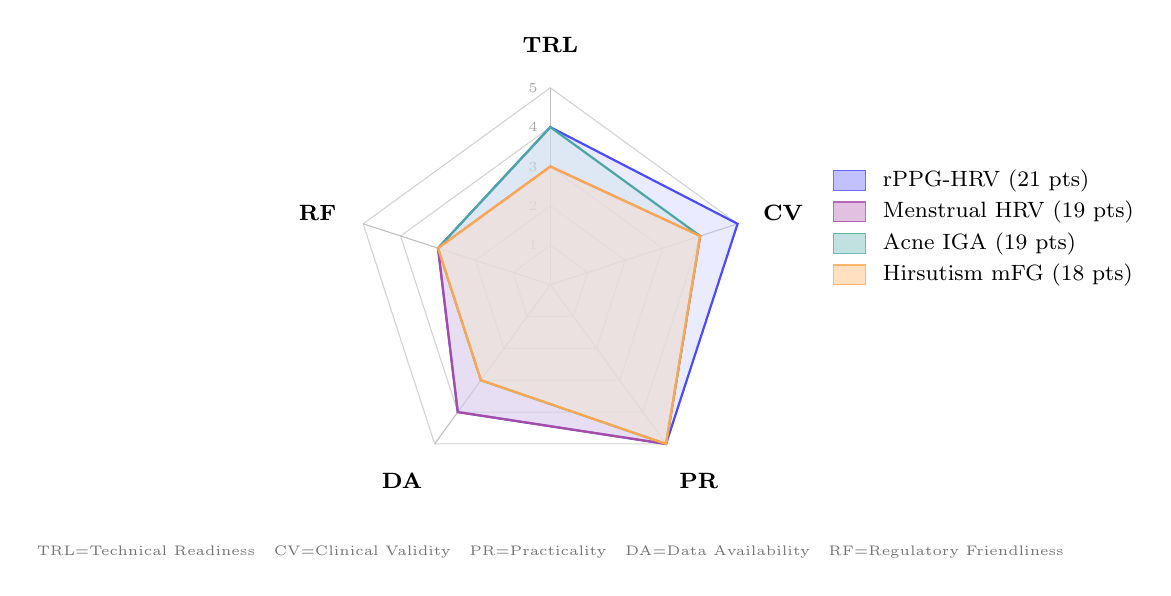
\begin{tikzpicture}[font=\small, >=Stealth]

\def\R{2.5}

\def\aTRL{90}
\def\aCV{18}
\def\aPR{306}
\def\aDA{234}
\def\aRF{162}

\foreach \s in {1,2,3,4,5}{
  \pgfmathsetmacro\r{\s/5*\R}
  \draw[gray!35, thin]
    ({\r*cos(\aTRL)},{\r*sin(\aTRL)}) --
    ({\r*cos(\aCV)}, {\r*sin(\aCV)})  --
    ({\r*cos(\aPR)}, {\r*sin(\aPR)})  --
    ({\r*cos(\aDA)}, {\r*sin(\aDA)})  --
    ({\r*cos(\aRF)}, {\r*sin(\aRF)})  -- cycle;
}

\foreach \a in {\aTRL,\aCV,\aPR,\aDA,\aRF}{
  \draw[gray!50] (0,0) -- ({\R*cos(\a)},{\R*sin(\a)});
}

\foreach \s/\lab in {1/1, 2/2, 3/3, 4/4, 5/5}{
  \pgfmathsetmacro\r{\s/5*\R}
  \node[font=\tiny, text=gray!70, left=1pt]
    at ({(\r)*cos(\aTRL)},{(\r)*sin(\aTRL)}) {\lab};
}

\pgfmathsetmacro\Rl{\R+0.45}
\node[align=center, font=\footnotesize\bfseries]
  at ({\Rl*cos(\aTRL)},{\Rl*sin(\aTRL)+0.1}) {TRL};
\node[align=center, font=\footnotesize\bfseries]
  at ({\Rl*cos(\aCV)+0.15},{\Rl*sin(\aCV)}) {CV};
\node[align=center, font=\footnotesize\bfseries]
  at ({\Rl*cos(\aPR)+0.15},{\Rl*sin(\aPR)-0.1}) {PR};
\node[align=center, font=\footnotesize\bfseries]
  at ({\Rl*cos(\aDA)-0.15},{\Rl*sin(\aDA)-0.1}) {DA};
\node[align=center, font=\footnotesize\bfseries]
  at ({\Rl*cos(\aRF)-0.15},{\Rl*sin(\aRF)}) {RF};

% B1 rPPG-HRV: 4,5,5,4,3
\pgfmathsetmacro\bOaTRL{4/5*\R} \pgfmathsetmacro\bOaCV{5/5*\R}
\pgfmathsetmacro\bOaPR{5/5*\R}  \pgfmathsetmacro\bOaDA{4/5*\R}
\pgfmathsetmacro\bOaRF{3/5*\R}
\filldraw[fill=blue!20, draw=blue!70, fill opacity=0.4, thick]
  ({\bOaTRL*cos(\aTRL)},{\bOaTRL*sin(\aTRL)}) --
  ({\bOaCV *cos(\aCV)}, {\bOaCV *sin(\aCV)})  --
  ({\bOaPR *cos(\aPR)}, {\bOaPR *sin(\aPR)})  --
  ({\bOaDA *cos(\aDA)}, {\bOaDA *sin(\aDA)})  --
  ({\bOaRF *cos(\aRF)}, {\bOaRF *sin(\aRF)})  -- cycle;

% B2 Menstrual HRV: 3,4,5,4,3
\pgfmathsetmacro\bTaTRL{3/5*\R} \pgfmathsetmacro\bTaCV{4/5*\R}
\pgfmathsetmacro\bTaPR{5/5*\R}  \pgfmathsetmacro\bTaDA{4/5*\R}
\pgfmathsetmacro\bTaRF{3/5*\R}
\filldraw[fill=violet!20, draw=violet!70, fill opacity=0.4, thick]
  ({\bTaTRL*cos(\aTRL)},{\bTaTRL*sin(\aTRL)}) --
  ({\bTaCV *cos(\aCV)}, {\bTaCV *sin(\aCV)})  --
  ({\bTaPR *cos(\aPR)}, {\bTaPR *sin(\aPR)})  --
  ({\bTaDA *cos(\aDA)}, {\bTaDA *sin(\aDA)})  --
  ({\bTaRF *cos(\aRF)}, {\bTaRF *sin(\aRF)})  -- cycle;

% B3 Acne IGA: 4,4,5,3,3
\pgfmathsetmacro\bRaTRL{4/5*\R} \pgfmathsetmacro\bRaCV{4/5*\R}
\pgfmathsetmacro\bRaPR{5/5*\R}  \pgfmathsetmacro\bRaDA{3/5*\R}
\pgfmathsetmacro\bRaRF{3/5*\R}
\filldraw[fill=teal!20, draw=teal!70, fill opacity=0.4, thick]
  ({\bRaTRL*cos(\aTRL)},{\bRaTRL*sin(\aTRL)}) --
  ({\bRaCV *cos(\aCV)}, {\bRaCV *sin(\aCV)})  --
  ({\bRaPR *cos(\aPR)}, {\bRaPR *sin(\aPR)})  --
  ({\bRaDA *cos(\aDA)}, {\bRaDA *sin(\aDA)})  --
  ({\bRaRF *cos(\aRF)}, {\bRaRF *sin(\aRF)})  -- cycle;

% B4 Hirsutism mFG: 3,4,5,3,3
\pgfmathsetmacro\bFaTRL{3/5*\R} \pgfmathsetmacro\bFaCV{4/5*\R}
\pgfmathsetmacro\bFaPR{5/5*\R}  \pgfmathsetmacro\bFaDA{3/5*\R}
\pgfmathsetmacro\bFaRF{3/5*\R}
\filldraw[fill=orange!20, draw=orange!70, fill opacity=0.4, thick]
  ({\bFaTRL*cos(\aTRL)},{\bFaTRL*sin(\aTRL)}) --
  ({\bFaCV *cos(\aCV)}, {\bFaCV *sin(\aCV)})  --
  ({\bFaPR *cos(\aPR)}, {\bFaPR *sin(\aPR)})  --
  ({\bFaDA *cos(\aDA)}, {\bFaDA *sin(\aDA)})  --
  ({\bFaRF *cos(\aRF)}, {\bFaRF *sin(\aRF)})  -- cycle;

\begin{scope}[xshift=3.6cm, yshift=1.2cm]
  \fill[blue!30,  draw=blue!70,  opacity=0.8] (0,0)    rectangle (0.4,0.25);
  \node[right, font=\footnotesize] at (0.5, 0.12)  {rPPG-HRV (21 pts)};
  \fill[violet!30,draw=violet!70, opacity=0.8] (0,-0.4) rectangle (0.4,-0.15);
  \node[right, font=\footnotesize] at (0.5,-0.28) {Menstrual HRV (19 pts)};
  \fill[teal!30,  draw=teal!70,   opacity=0.8] (0,-0.8) rectangle (0.4,-0.55);
  \node[right, font=\footnotesize] at (0.5,-0.68) {Acne IGA (19 pts)};
  \fill[orange!30,draw=orange!70, opacity=0.8] (0,-1.2) rectangle (0.4,-0.95);
  \node[right, font=\footnotesize] at (0.5,-1.08){Hirsutism mFG (18 pts)};
\end{scope}

\node[font=\tiny, align=center, text=black!55, yshift=-0.3cm] at (0,-3.1) {%
  TRL=Technical Readiness\quad CV=Clinical Validity\quad
  PR=Practicality\quad DA=Data Availability\quad RF=Regulatory Friendliness};

\end{tikzpicture}
\caption{Five-dimensional radar chart for Tier~1 biomarker evaluation.
Each axis represents one evaluation dimension scored 1--5.
All four Tier~1 biomarkers score 5/5 on Practicality (PR), reflecting
direct collectability via standard smartphone cameras without additional hardware.
rPPG-HRV leads overall (21/25) due to its high Clinical Validity (meta-analytic
evidence) and partial regulatory precedent (FDA-cleared FibriCheck).}
\label{fig:radar}
\end{figure*}
% ────────────────────────────────────────────────────────────────────────────

\subsection{Five-Dimensional Priority Matrix for Tier~1 Biomarkers}

Table~\ref{tab:priority} provides detailed assessment of each Tier~1 biomarker across the five evaluation dimensions, including supporting evidence and key limitations.

\begin{table*}[t]
\centering
\caption{Five-Dimensional Priority Assessment of Tier~1 Biomarkers}
\label{tab:priority}
\begin{tabular}{p{2.8cm}p{2.5cm}p{2.5cm}p{2.5cm}p{2.5cm}p{2.5cm}}
\toprule
\textbf{Biomarker} & \textbf{TRL} & \textbf{Clinical Validity} & \textbf{Practicality} & \textbf{Data Availability} & \textbf{Regulatory} \\
\midrule
rPPG-HRV & Public models, real-world validated~\cite{debnath2025comprehensive} & Meta-analysis: 17 studies, High evidence~\cite{Mirzohreh_2024} & 60s video, any smartphone & UBFC-rPPG, PURE benchmarks & FibriCheck FDA-cleared (AF)~\cite{Sollee_2025} \\
\addlinespace
Menstrual HRV Pattern & Wearable-validated, rPPG transfer needed & Living SR~\cite{de_Jager_2026}, large-scale~\cite{Heydari_2025} & Daily 60s + app logging & App data + rPPG longitudinal & SaMD precedents exist \\
\addlinespace
Acne IGA & AcneDet~\cite{Huynh_2022}, AcneAI~\cite{Gazeau_2024} & IGA 0.85, ICC 0.8; PCOS-androgen link & Standard selfie & ACNE04 dataset, clinical & Class~I SaMD pathway \\
\addlinespace
Hirsutism mFG & Image-based validation~\cite{Oliveira_2022} & $r=0.89$, $\kappa=0.75$; Rotterdam criterion & Targeted photos & Limited public data & Screening tool pathway \\
\bottomrule
\end{tabular}
\end{table*}

\subsection{Meta-Analytic Performance Summary}

Table~\ref{tab:meta} synthesizes existing performance data from the literature to project expected performance of individual and combined modalities for PCOS and endometriosis classification.

\begin{table}[t]
\centering
\caption{Performance Meta-Analysis and Projected Multimodal Fusion AUC}
\label{tab:meta}
\begin{tabular}{lcccc}
\toprule
\textbf{Modality} & \textbf{PCOS} & \textbf{Endo} & \textbf{3-class} & \textbf{Evidence} \\
\midrule
rPPG-HRV only & 0.70--0.80 & 0.65--0.75 & 0.65--0.75 & High \\
Skin analysis only & 0.75--0.85 & 0.55--0.65 & 0.60--0.70 & Moderate \\
Menstrual only & 0.65--0.75 & 0.60--0.70 & 0.60--0.70 & Moderate \\
\textbf{Fusion (all)} & \textbf{0.85--0.90} & \textbf{0.75--0.85} & \textbf{0.80--0.90} & Projected \\
\bottomrule
\end{tabular}
\end{table}

The projected advantage of multimodal fusion arises from the complementary nature of the three modalities. rPPG-HRV captures autonomic dysregulation common to both conditions but with distinct signatures: sympathetic overactivation in PCOS (elevated LF/HF) versus vagal tone reduction in endometriosis (decreased RMSSD, HF)~\cite{Mirzohreh_2024, Hao_2021}. Skin phenotype analysis is highly specific to PCOS (acne, hirsutism, acanthosis nigricans) but contributes minimally to endometriosis detection. Menstrual pattern analysis provides complementary information: irregular cycles characteristic of PCOS anovulation and pain patterns specific to endometriosis. Cross-Attention Fusion enables the model to learn these disease-specific feature interactions.

We emphasize that the fusion AUC estimates are projections based on individual modality performance and published multimodal fusion gains in analogous domains; they require empirical validation through the proposed cohort study.

\subsection{Differentiation from Prior Work}

Our prior systematic review~\cite{debnath2025comprehensive, rppgreview2024frontiers} established a comprehensive taxonomy of smartphone camera-based biomarkers across six technology domains but addressed no specific disease focus. The present work differs in four fundamental ways: (1) \textit{disease-specific targeting} of PCOS and endometriosis rather than broad technology cataloging; (2) \textit{multimodal framework design} combining three complementary modalities through learned attention mechanisms; (3) \textit{diagnostic delay-centered narrative} grounding clinical motivation in the 7--10 year delay problem; and (4) \textit{concrete validation protocol} with power-justified sample sizes derived from disease-specific meta-analytic effect sizes.

%==============================================================================
\section{Discussion}
%==============================================================================

\subsection{Technical Challenges}

\subsubsection{PCOS Phenotypic Heterogeneity}
PCOS manifests in multiple phenotypes---hyperandrogenic, metabolic, lean, and mixed---each with distinct biomarker profiles~\cite{Wang_2025, Bernal_2024}. The classic hyperandrogenic phenotype with acne, hirsutism, and elevated BMI would produce strong DermScore signals, whereas lean PCOS may manifest only through HRV alterations and menstrual irregularity. Our Cross-Attention Fusion architecture addresses this by learning phenotype-dependent feature weighting, but adequate representation of each phenotype in the training cohort is essential. We recommend stratified enrollment targeting equal representation of at least three phenotypic subtypes.

\subsubsection{Endometriosis Phenotypic Diversity}
Endometriosis encompasses superficial peritoneal, ovarian endometrioma, and deep infiltrating subtypes across rASRM stages I--IV, with varying symptom profiles and likely different autonomic signatures~\cite{Zeng_2025, Moreira_2024}. Stage I--II disease may produce subtle HRV changes below rPPG detection thresholds, while deep infiltrating endometriosis with severe pain may generate stronger vagal suppression signals~\cite{Moreira_2021}. Stage-stratified subgroup analysis is planned for Phase~II to characterize this heterogeneity.

\subsubsection{rPPG Signal Quality in Real-World Conditions}
Acharya et al.~\cite{acharya2025reliability} demonstrated that rPPG reliability degrades significantly under low illumination ($<$50 lux) and elevated heart rate. Our protocol mitigates this through standardized indoor capture with automatic ambient light verification (50--500 lux), the CHROM+DeepPhys hybrid approach for robustness, and SQI-based quality filtering. The Phase~I pilot will quantify the proportion of rejected sessions and refine capture guidelines accordingly.

\subsection{Women's Health Equity and Diagnostic Equity}

The 7--10 year diagnostic delay for endometriosis represents a systemic failure in women's healthcare~\cite{Pavic_2025, Zhang_2026}. Contributing factors include normalization of menstrual pain, limited access to specialist gynecological care, and the absence of non-invasive screening tools. Our framework directly addresses diagnostic equity by offering a population-level screening pathway that requires only a smartphone, potentially reaching women in primary care settings, rural areas, and low-resource countries.

PCOS similarly suffers from diagnostic inequity, with studies showing that women of lower socioeconomic status and racial/ethnic minorities face longer times to diagnosis~\cite{Arabkermani_2025}. The smartphone-based approach could reduce these disparities if validated across diverse populations.

\subsubsection{Skin Tone Bias Mitigation}
rPPG accuracy is known to degrade for darker skin tones (Fitzpatrick types V--VI)~\cite{Sollee_2025}. Our protocol addresses this through: (1) mandatory Fitzpatrick type recording at enrollment; (2) stratified analysis by skin type with pre-specified equivalence margins ($\Delta$AUC $<$ 0.05); (3) adaptive ROI selection that adjusts to melanin-related signal attenuation; and (4) targeted enrollment to ensure adequate representation of darker skin tones ($\geq$20\% Fitzpatrick V--VI).

\subsection{Privacy-by-Design Principles}

Facial images and video contain biometric data requiring stringent privacy protections. Our framework implements a three-layer privacy architecture: (1) \textit{On-device processing}: rPPG signal extraction occurs on the smartphone, with raw video deleted immediately after HRV computation; skin analysis extracts only the 16-dimensional DermScore vector, with original photographs never transmitted; (2) \textit{Federated learning option}: model parameters are exchanged during training without raw data migration, enabling multi-institutional collaboration while preserving data sovereignty; (3) \textit{Regulatory compliance}: the protocol adheres to GDPR, Korean Personal Information Protection Act (PIPA), and HIPAA requirements for health data handling, with explicit informed consent for facial image capture, defined retention periods, and guaranteed deletion procedures.

\subsection{Limitations and Future Work}

Several limitations warrant acknowledgment. First, the projected fusion AUC of 0.80--0.90 remains unvalidated; actual performance may be lower due to noise accumulation across modalities and population heterogeneity. Second, the framework currently excludes women with PCOS-endometriosis comorbidity (estimated 7--15\% overlap), who represent a clinically important subgroup requiring future investigation. Third, longitudinal compliance over multiple menstrual cycles may limit the practical feasibility of Module~C, particularly for endometriosis patients experiencing significant pain. Fourth, our evaluation relies on reference diagnoses (Rotterdam criteria, laparoscopy) that themselves have imperfect sensitivity, introducing label noise into the training data. Finally, the framework is designed as a screening tool to prioritize women for clinical evaluation, not as a stand-alone diagnostic---integration with existing clinical workflows requires careful implementation research.

Future work will encompass Phase~I pilot execution, development of an open-source rPPG-HRV extraction toolkit optimized for women's health applications, extension to adolescent populations (where early detection has the greatest impact), and integration of additional biomarkers from Tier~2 and Tier~3 candidates as technical maturity advances.

%==============================================================================
\section{Conclusion}
%==============================================================================

We have presented the first smartphone camera-based multimodal biomarker framework specifically designed for AI-driven prediction of PCOS and endometriosis---two conditions that collectively affect hundreds of millions of women yet remain severely underdiagnosed due to reliance on invasive procedures and specialist access. By synthesizing convergent evidence from three domains (rPPG-HRV autonomic sensing, AI-driven skin phenotype analysis, and digital menstrual cycle tracking), we identified four Tier~1 biomarkers with both strong clinical evidence and mature smartphone camera technology. Our proposed Cross-Attention Fusion architecture enables disease-specific feature interaction learning while gracefully handling missing modalities.

The three-phase cohort protocol, grounded in meta-analytic effect sizes and powered for clinically meaningful performance targets, provides a concrete validation pathway. Equally importantly, our framework embeds diagnostic equity principles---smartphone accessibility, skin tone bias mitigation, and Privacy-by-Design---that are essential for any technology aspiring to reduce the 7--10 year diagnostic delay experienced by women worldwide.

This work establishes smartphone camera-based multimodal biomarkers as a viable and scientifically grounded approach to non-invasive PCOS and endometriosis screening. Successful validation would represent a paradigm shift from episodic, facility-based diagnosis to continuous, patient-centered health monitoring, potentially transforming the landscape of women's reproductive healthcare.

\bibliographystyle{IEEEtran}
\bibliography{references}

\end{document}
